\section{Details of Meta Evaluation}
\label{appendix:meta_evaluation}
\begin{figure}[ht]
    \centering    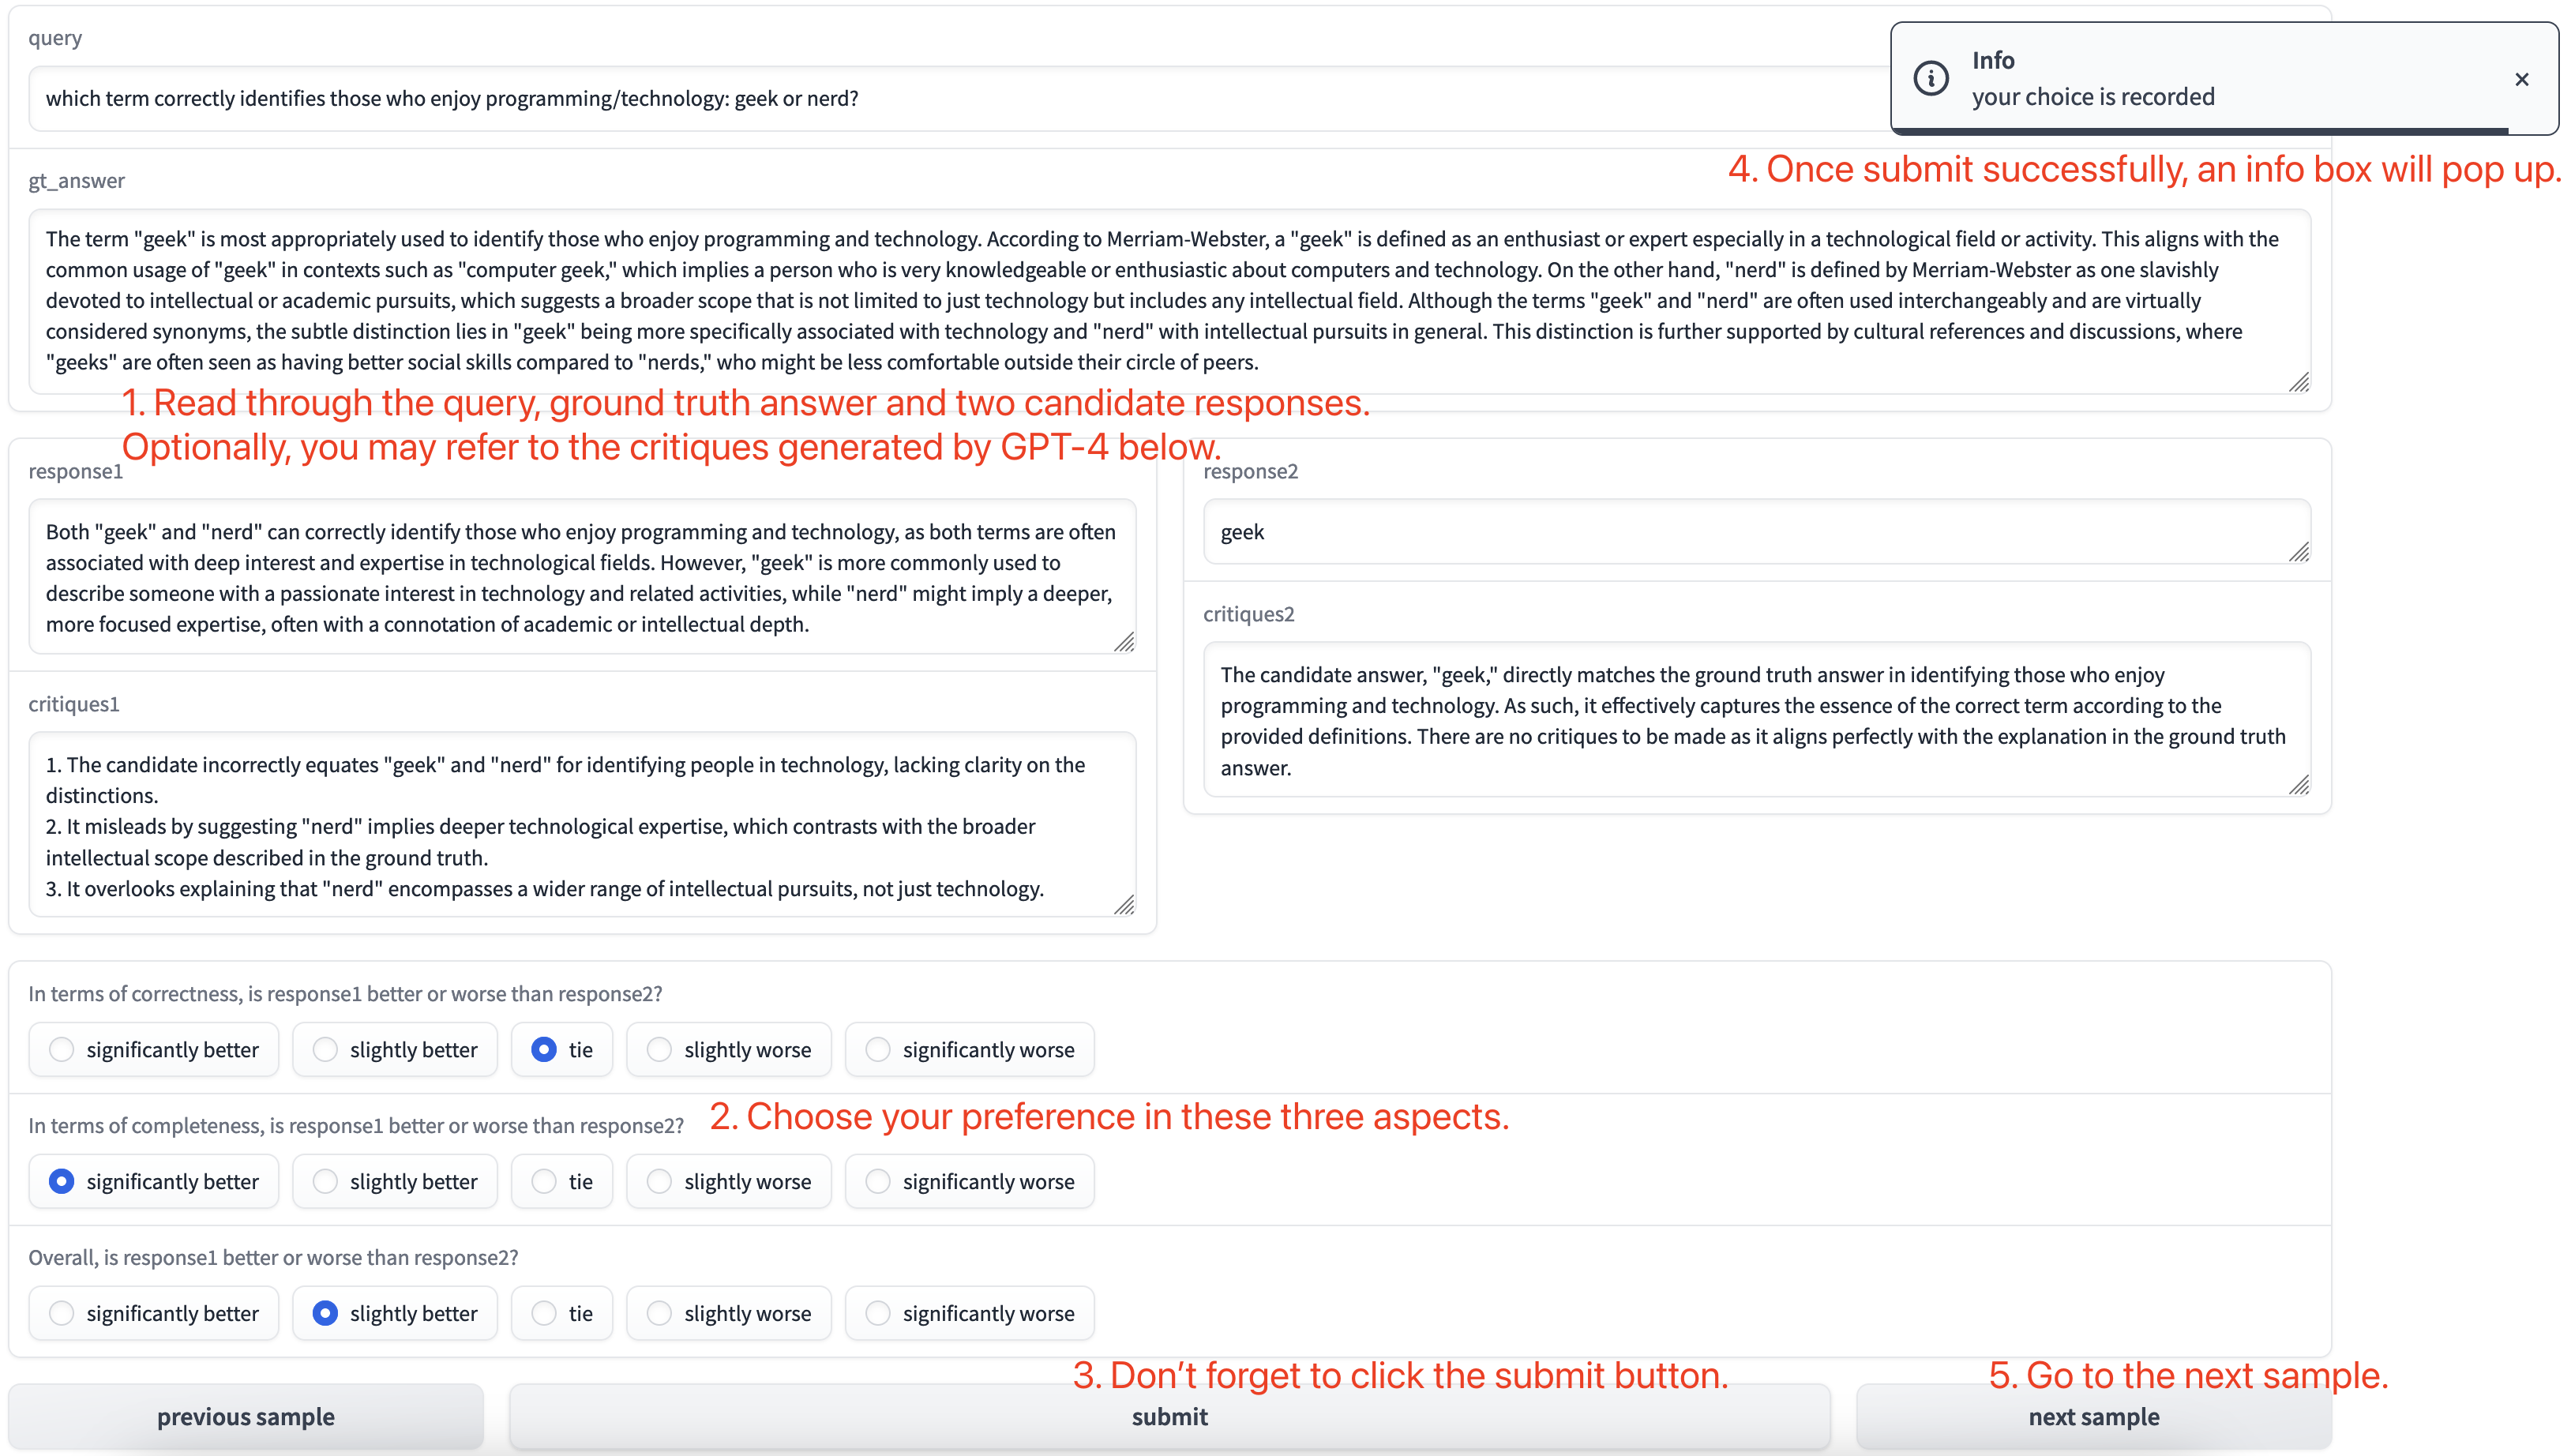
\includegraphics[width=\textwidth]{figures/annotation_tool.png}
    \caption[]{The human annotation interface and instructions of the meta evaluation dataset.}
    \label{fig:annotation_tool}
\end{figure}

In the meta evaluation, we ask 10 annotators compare two responses from the RAG system for each instance in the meta evaluation dataset. Seven of the annotators are in-house annotators, and three of them are graduate students. We pay the students 15 USD per hour and totally cost 255 dollars.

Annotators are required to choose their preference from five options: significantly better, slightly better, tie, slightly worse, or significantly worse. The annotation is based on three metrics: correctness, completeness, and overall assessment. The annotation interface with instructions are shown in Fig.~\ref{fig:annotation_tool}

To make sure the human evaluation to be agnostic to specific evaluation metrics, we provide the annotators with a detailed annotation guideline which contains detailed instruction and 5 examples. In the UI of the annotation tool, each response is shown with critiques generated by GPT-4 and we ask the annotators to refer to the content of the response and the critiques for labeling. The critiques are generated by prompting GPT-4 to compare the response with ground truth answer to ease the annotation job. In addition, each of the example the guideline are shown with a human-written explanation for the labeling. 


The 10 metrics included in the meta evaluation are selected from Trulens~\cite{TruLens}, RAGAS~\cite{es2023ragas}, ARES~\cite{saadfalcon2023ares} and CRUD-RAG~\cite{lyu2024crud} as explained in Sec.~\ref{sec:meta_evaluation}. Their descriptions are summarized in Tab.~\ref{tab:baseline_metrics}.
As a supplement of Tab.~\ref{tab:meta_evaluation_selected}, the full correlation results of meta evaluation is shown in Tab.~\ref{tab:meta_evaluation_full}.
For a detailed comparison between \benchname\space and the strongest baseline metric, RAGAS Answer Similarity, we plot the prediction score distribution of two metrics in Fig.~\ref{fig:ragchecker_vs_ragas}. From the prediction score distribution and the mean line (dashed line) of the plot, we can observe a stronger correlation of \benchname\space than RAGAS Answer Similarity.

\begin{table}[htbp]
  \centering
  \renewcommand{\arraystretch}{1.5}
  \caption{Summary of the metrics included in the meta evaluation.}
  \label{tab:baseline_metrics}
  \scalebox{0.8}{
  \begin{tabular}{>{\centering\arraybackslash}m{2cm}|>{\centering\arraybackslash}m{3cm}|>{\centering\arraybackslash}m{9cm}}
    \hline
    \textbf{Baseline} & \textbf{Metric} & \textbf{Description} \\
    \hline
    \multirow{2}{*}{\raisebox{-1.5ex}{TruLens}} & Groundedness & Assesses the overlap between each statement in the response and the provided context using an LLM. \\\cline{2-3}
                                                & Answer Relevance & Prompts an LLM to give a relevance score between the response and question. \\\hline
    \multirow{4}{*}{\raisebox{-10ex}{RAGAS}}  & Faithfulness & Measures the proportion of claims in the response that can be inferred from the context. \\\cline{2-3}
                                                & Answer Relevance & Computes the mean cosine similarity between the original question and a series of LLM-generated questions derived from the response and context. \\\cline{2-3}
                                                & Answer Similarity & Measures the semantic similarity between the response and the ground truth answer based on text-embedding-ada-002~\cite{neelakantan2022text}. \\\cline{2-3}
                                                & Answer Correctness & Quantifies both the semantic similarity and the factual overlap between the response and the ground truth answer. \\\hline
    \multirow{2}{*}{\raisebox{-5ex}{ARES}}   & Answer Faithfulness & Prompts an LLM to determine whether the response is faithful to the context. \\\cline{2-3}
                                                & Answer Relevance & Prompts an LLM to measure whether the response addresses all aspects of the question and provides only correct information from the context.  \\\hline
    \multirow{2}{*}{\raisebox{-1.5ex}{CRUD-RAG}} & Recall & Computes the ratio of all questions generated from ground truth answers that can be answered by response.\\\cline{2-3}
                                                 & Precision & Evaluates if the generated text is accurate and consistent with the ground truth answer.\\
    \hline
  \end{tabular}
  }
\end{table}

\begin{table}[htbp]
  \centering
  \caption{Full Correlation results with Human Evaluation of Correctness, Completeness, and Overall Assessment}
  \scalebox{0.83}{
  \begin{tabular}{lccccccc}
    \toprule
    \multirow{2.5}{*}{\textbf{Baseline}} & 
    \multirow{2.5}{*}{\textbf{Metric}} & 
    \multicolumn{2}{c}{\textbf{Correctness}} & 
    \multicolumn{2}{c}{\textbf{Completeness}} & 
    \multicolumn{2}{c}{\textbf{Overall Assessment}} \\
    \cmidrule(lr){3-4} \cmidrule(lr){5-6} \cmidrule(lr){7-8}
    & & \textbf{Pearson} & \textbf{Spearman} & \textbf{Pearson} & \textbf{Spearman} & \textbf{Pearson} & \textbf{Spearman} \\
    \midrule
    BLEU& BLEU-avg & 38.89 & 35.32 & 32.13 & 21.85 & 35.14 & 29.42 \\
    ROUGE& ROUGE-L & 31.75 & 31.72 & 47.88 & 45.67 & 43.10 & 43.21 \\
    BERTScore& BERTScore & 30.34 & 27.05 & 37.93 & 40.05 & 33.51 & 35.57 \\
    TruLens & Groundedness & 21.11 & 18.21 & 14.01 & 6.02 & 19.45 & 14.42 \\
    TruLens & Answer Relevance & 35.01 & 27.37 & 37.24 & 37.91 & 35.15 & 33.59 \\
    ARES & Answer Relevance & 18.63 & 16.84 & 20.13 & 18.13 & 17.81 & 16.26 \\
    ARES & Answer Faithfulness & 9.46 & 7.60 & 10.25 & 8.99 & 8.80 & 7.58 \\
    RAGAS & Faithfulness & 8.22 & 7.53 & 4.90 & 1.19 & 7.83 & 5.55 \\
    RAGAS & Answer Correctness & 39.11 & 36.30 & 36.42 & 36.04 & 38.01 & 37.14 \\
    RAGAS & Answer Similarity & \underline{41.07} & \underline{43.21} & \underline{53.16} & \textbf{61.35} & \underline{48.31} & \underline{57.23} \\
    RAGAS & Answer Relevance & 11.59 & 8.19 & 9.39 & 13.57 & 10.27 & 11.83 \\
    CRUD-RAG & Precision & 20.73 & 15.67 & 25.58 & 20.33 & 25.59 & 19.63 \\
    CRUD-RAG & Recall & 30.93 & 27.13 & 45.11 & 43.76 & 41.25 & 39.71 \\
    RAGChecker & Same metric as human & \textbf{49.66} & \textbf{46.95} & \textbf{60.67} & \underline{58.11} & \textbf{61.93} & \textbf{60.90} \\
    \midrule
    Human & Annotator sanity check & 63.67 & 59.19 & 71.91 & 68.36 & 70.09 & 68.89 \\
    \bottomrule
  \end{tabular}
  }
  \label{tab:meta_evaluation_full}
\end{table}



\begin{figure}
\centering
\begin{subfigure}{.7\textwidth}
  \centering
  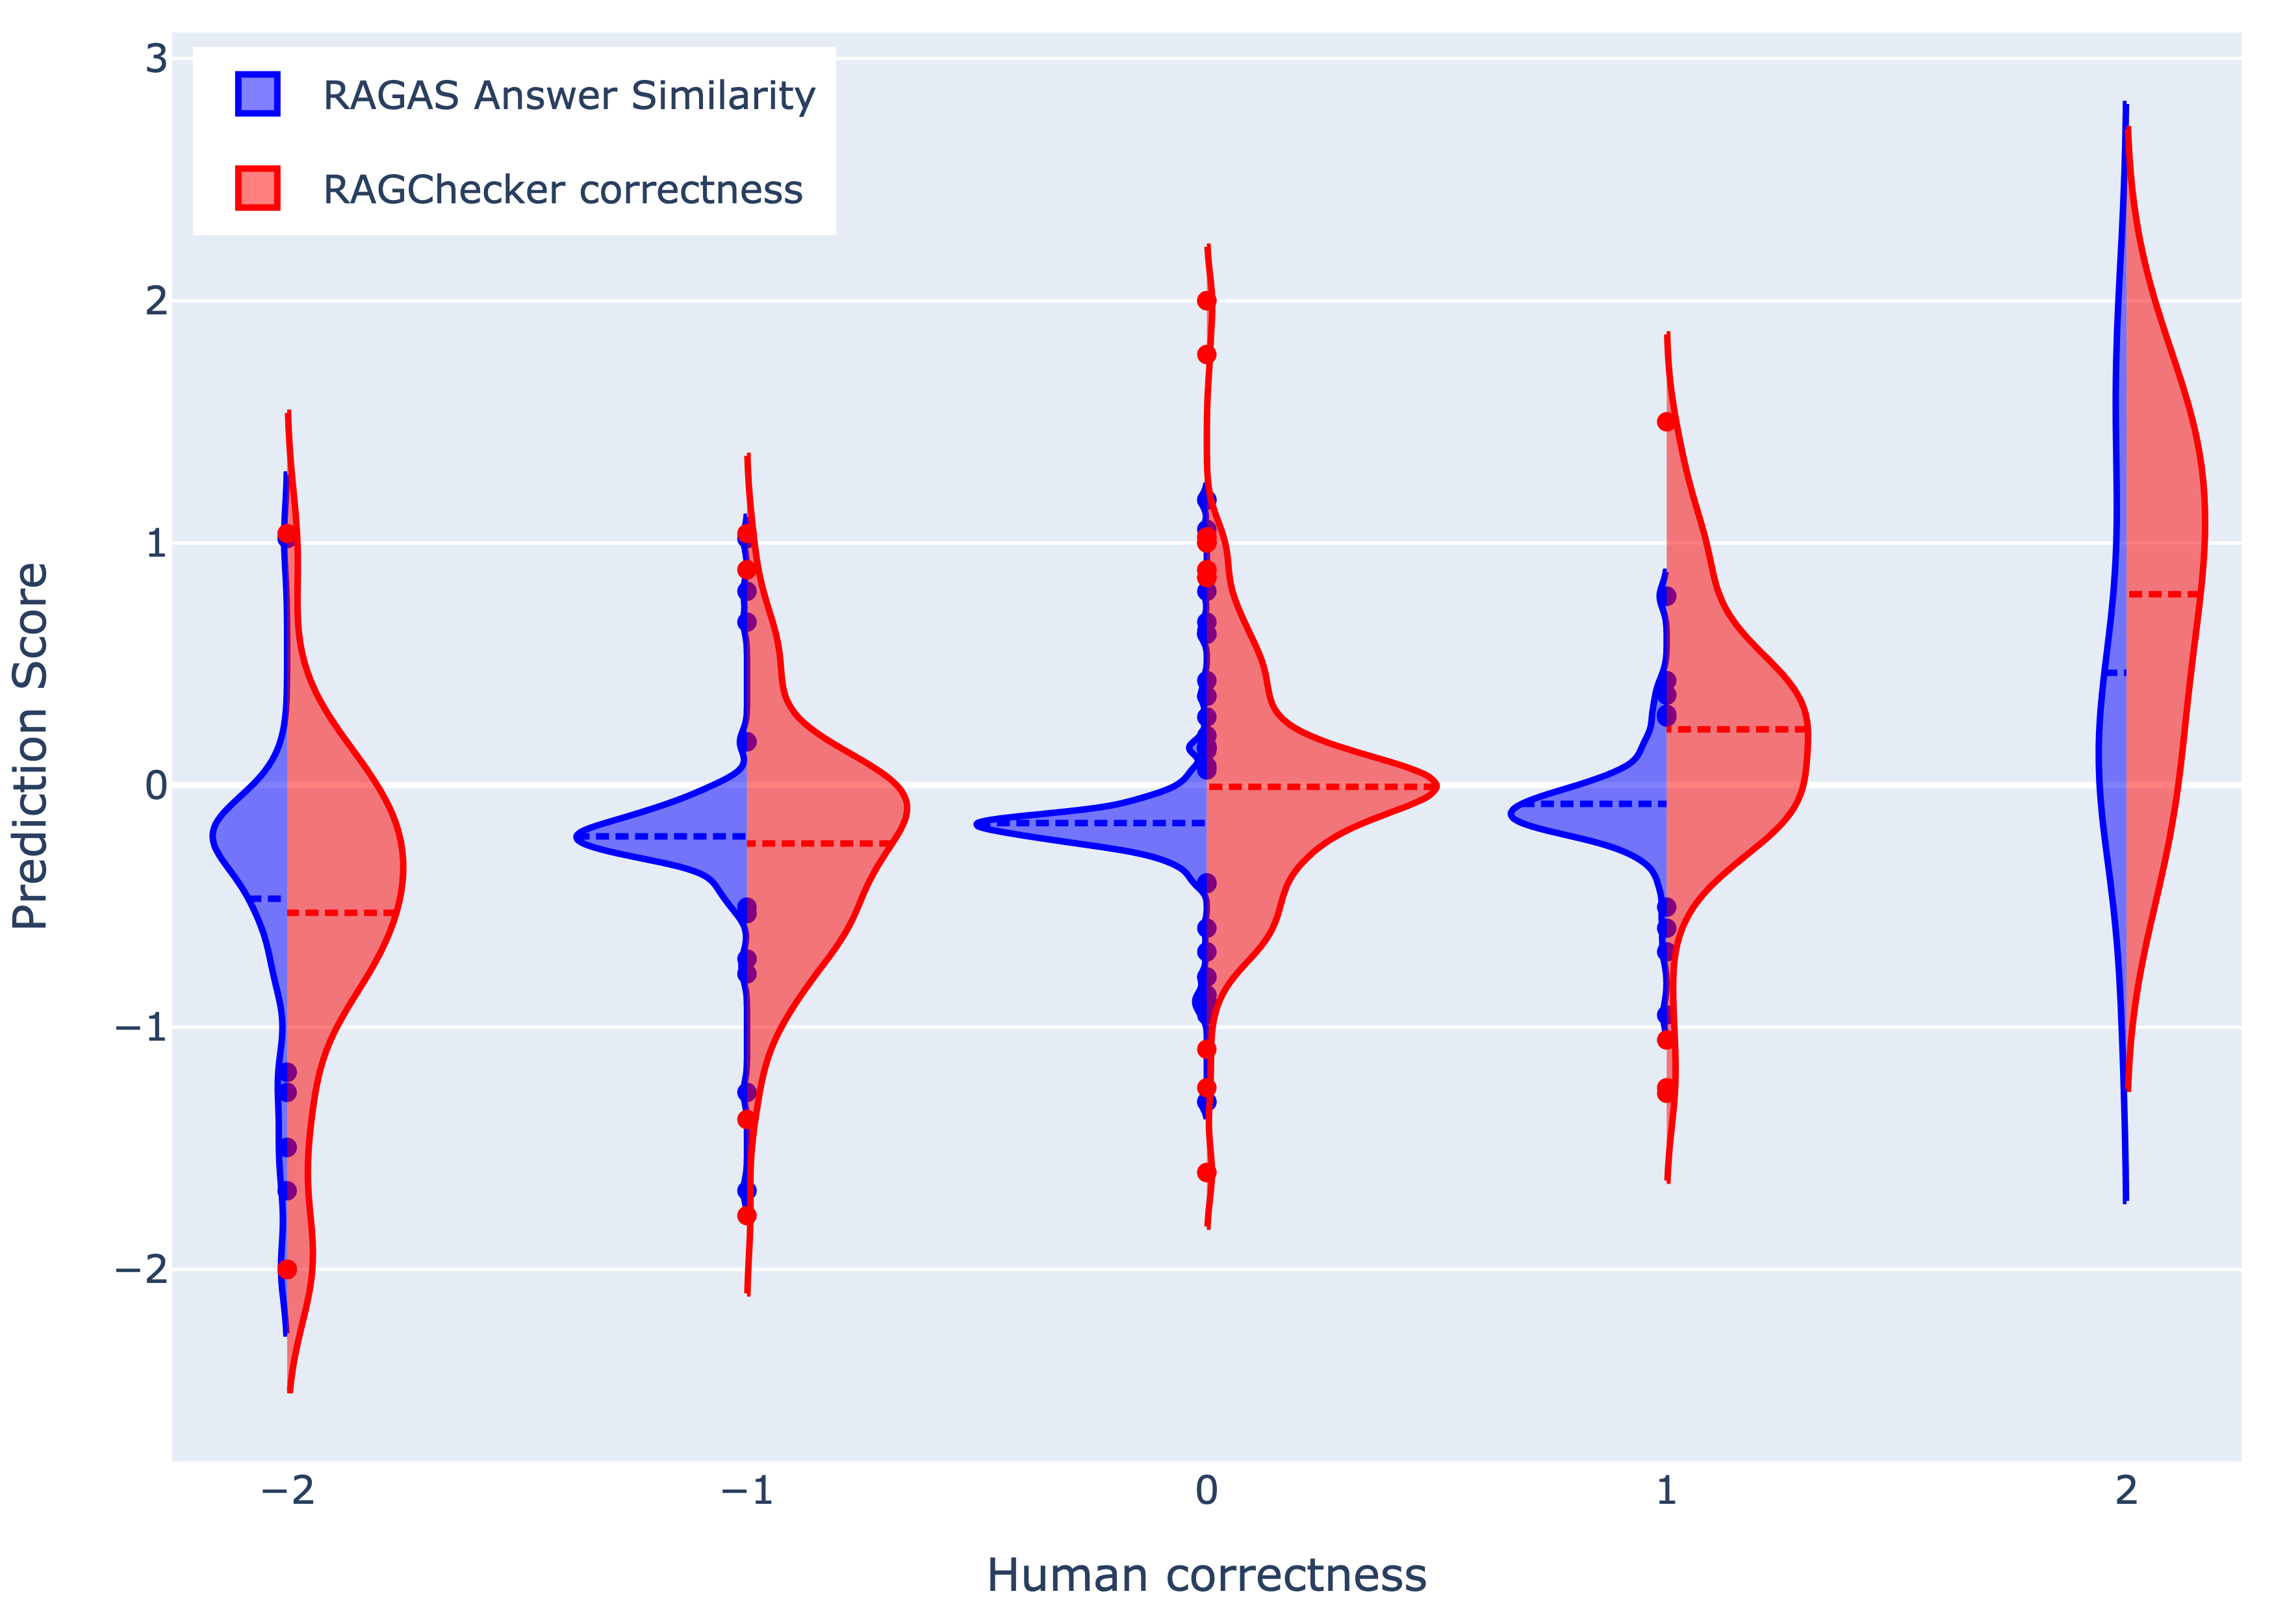
\includegraphics[width=\linewidth]{figures/human_correctness.png}
\end{subfigure}
\begin{subfigure}{.7\textwidth}
  \centering
  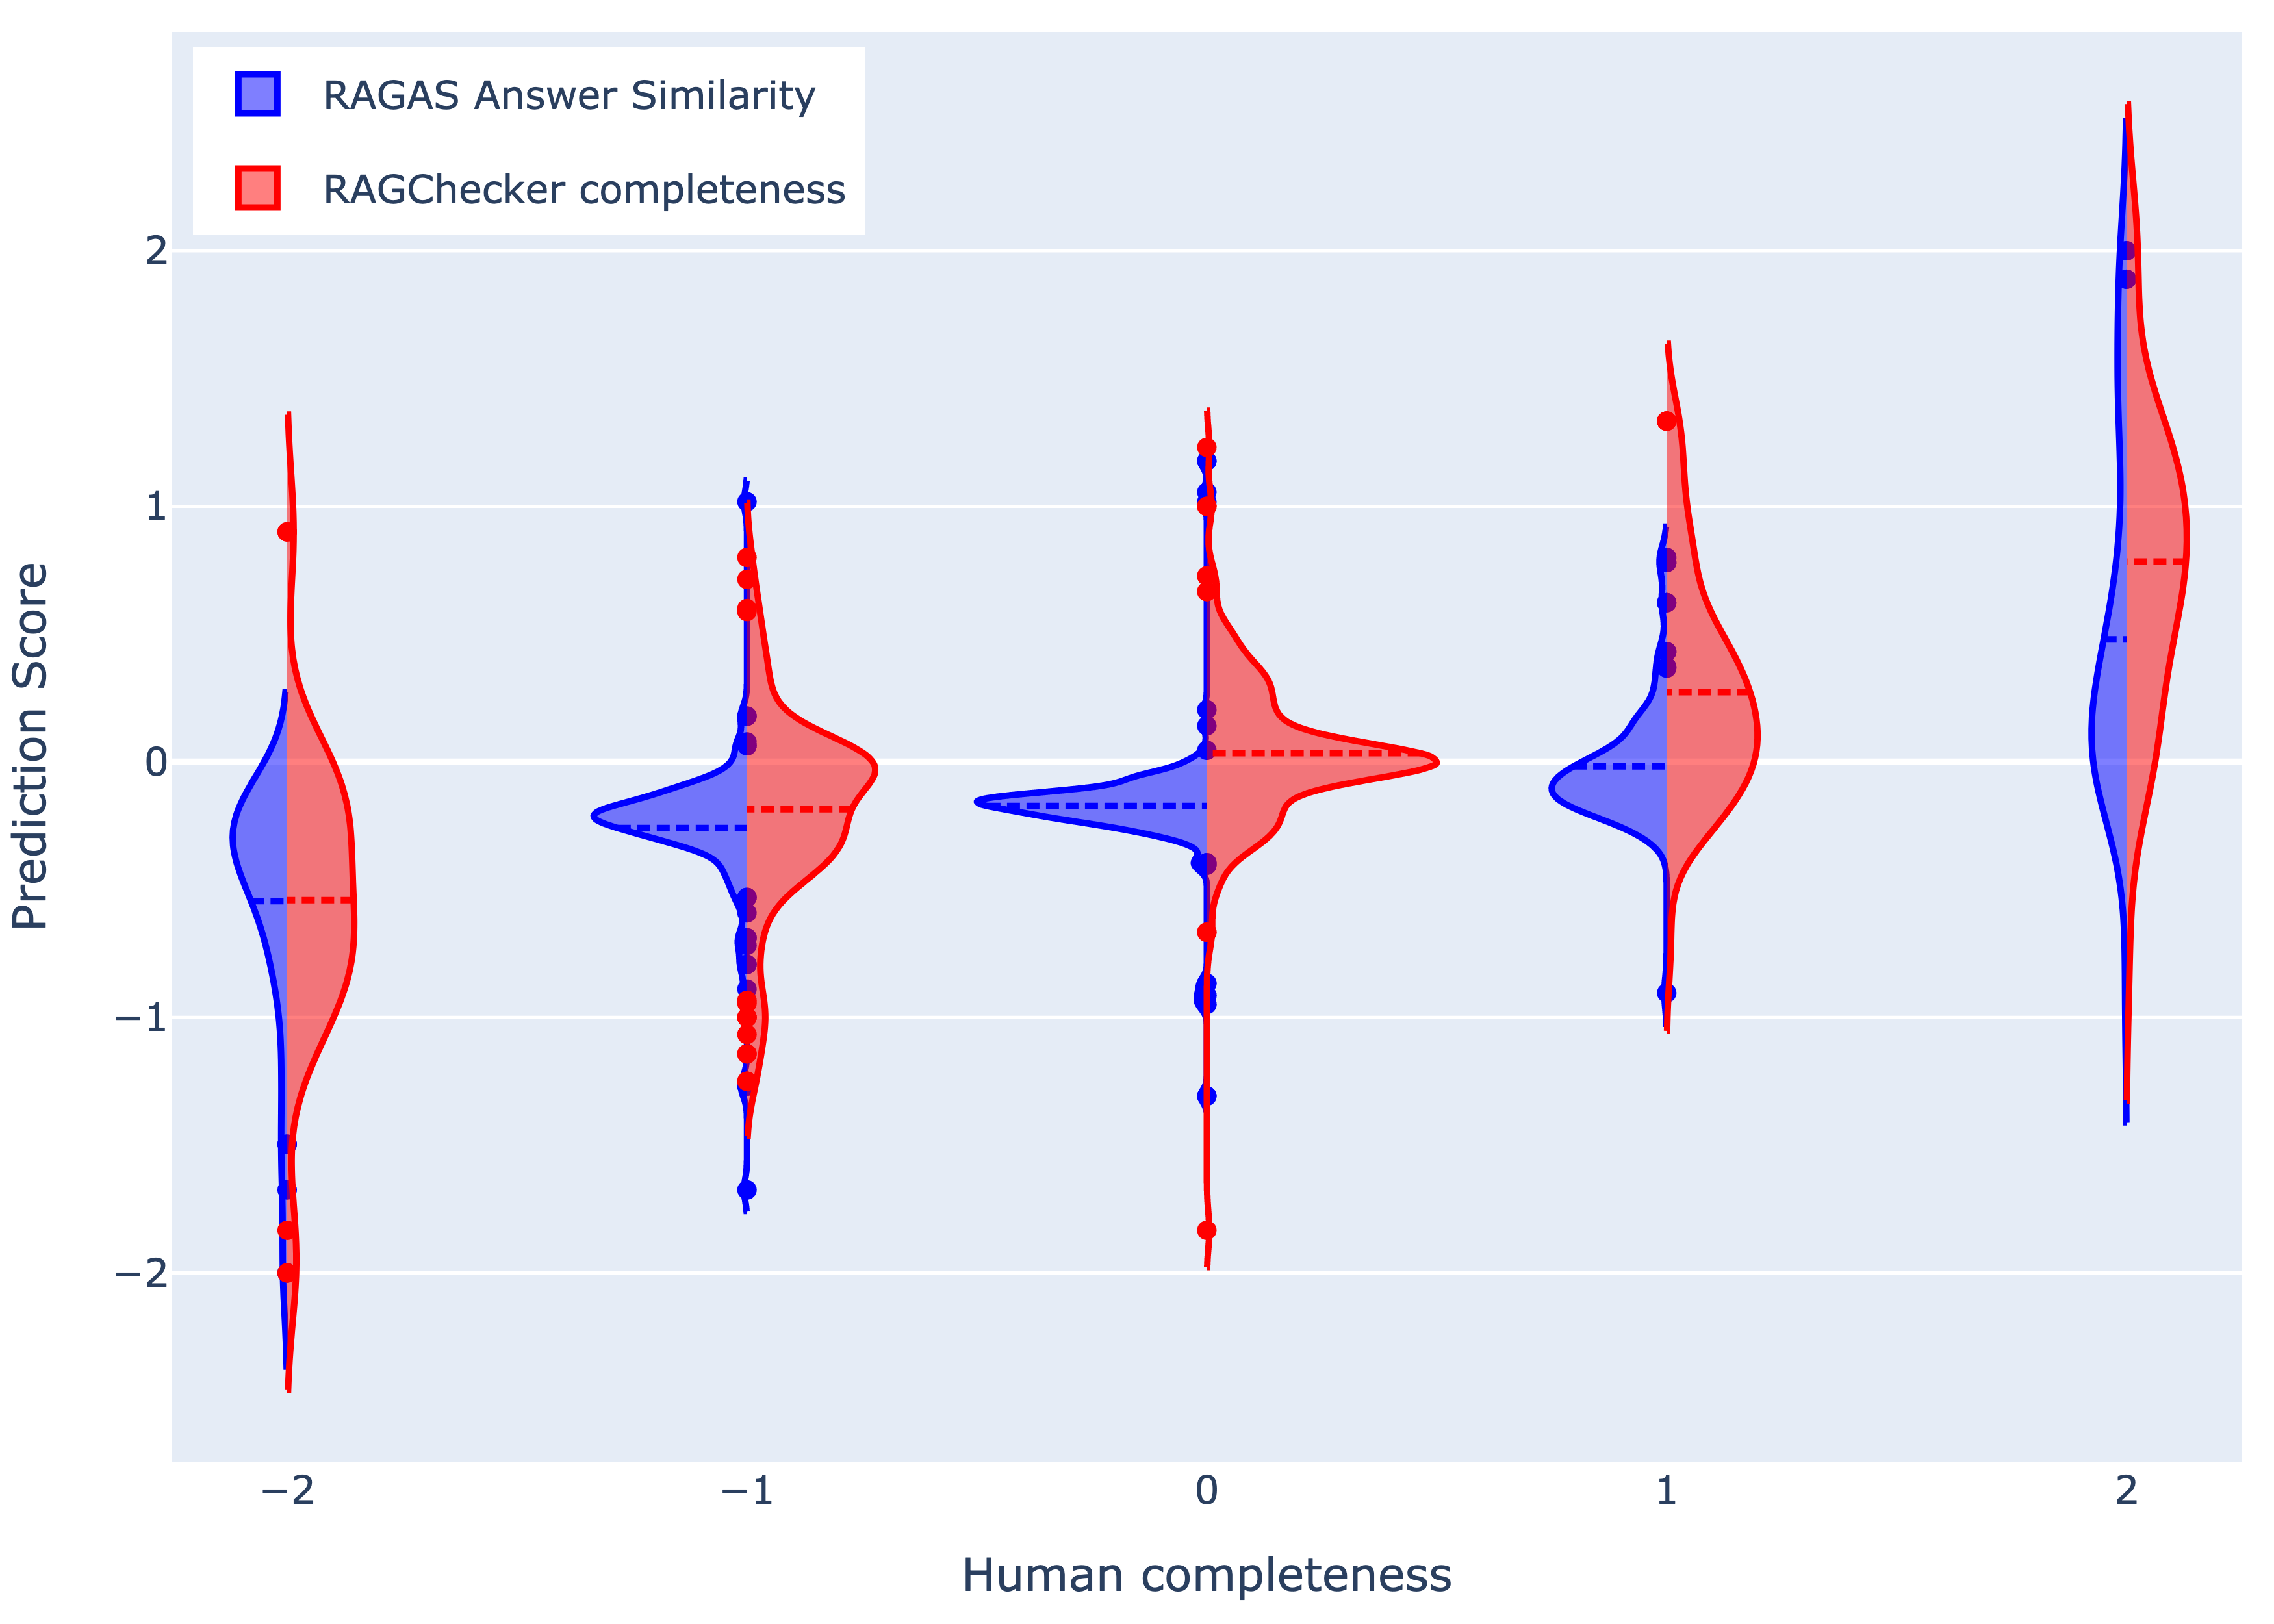
\includegraphics[width=\linewidth]{figures/human_completeness.png}
\end{subfigure}
\begin{subfigure}{.7\textwidth}
  \centering
  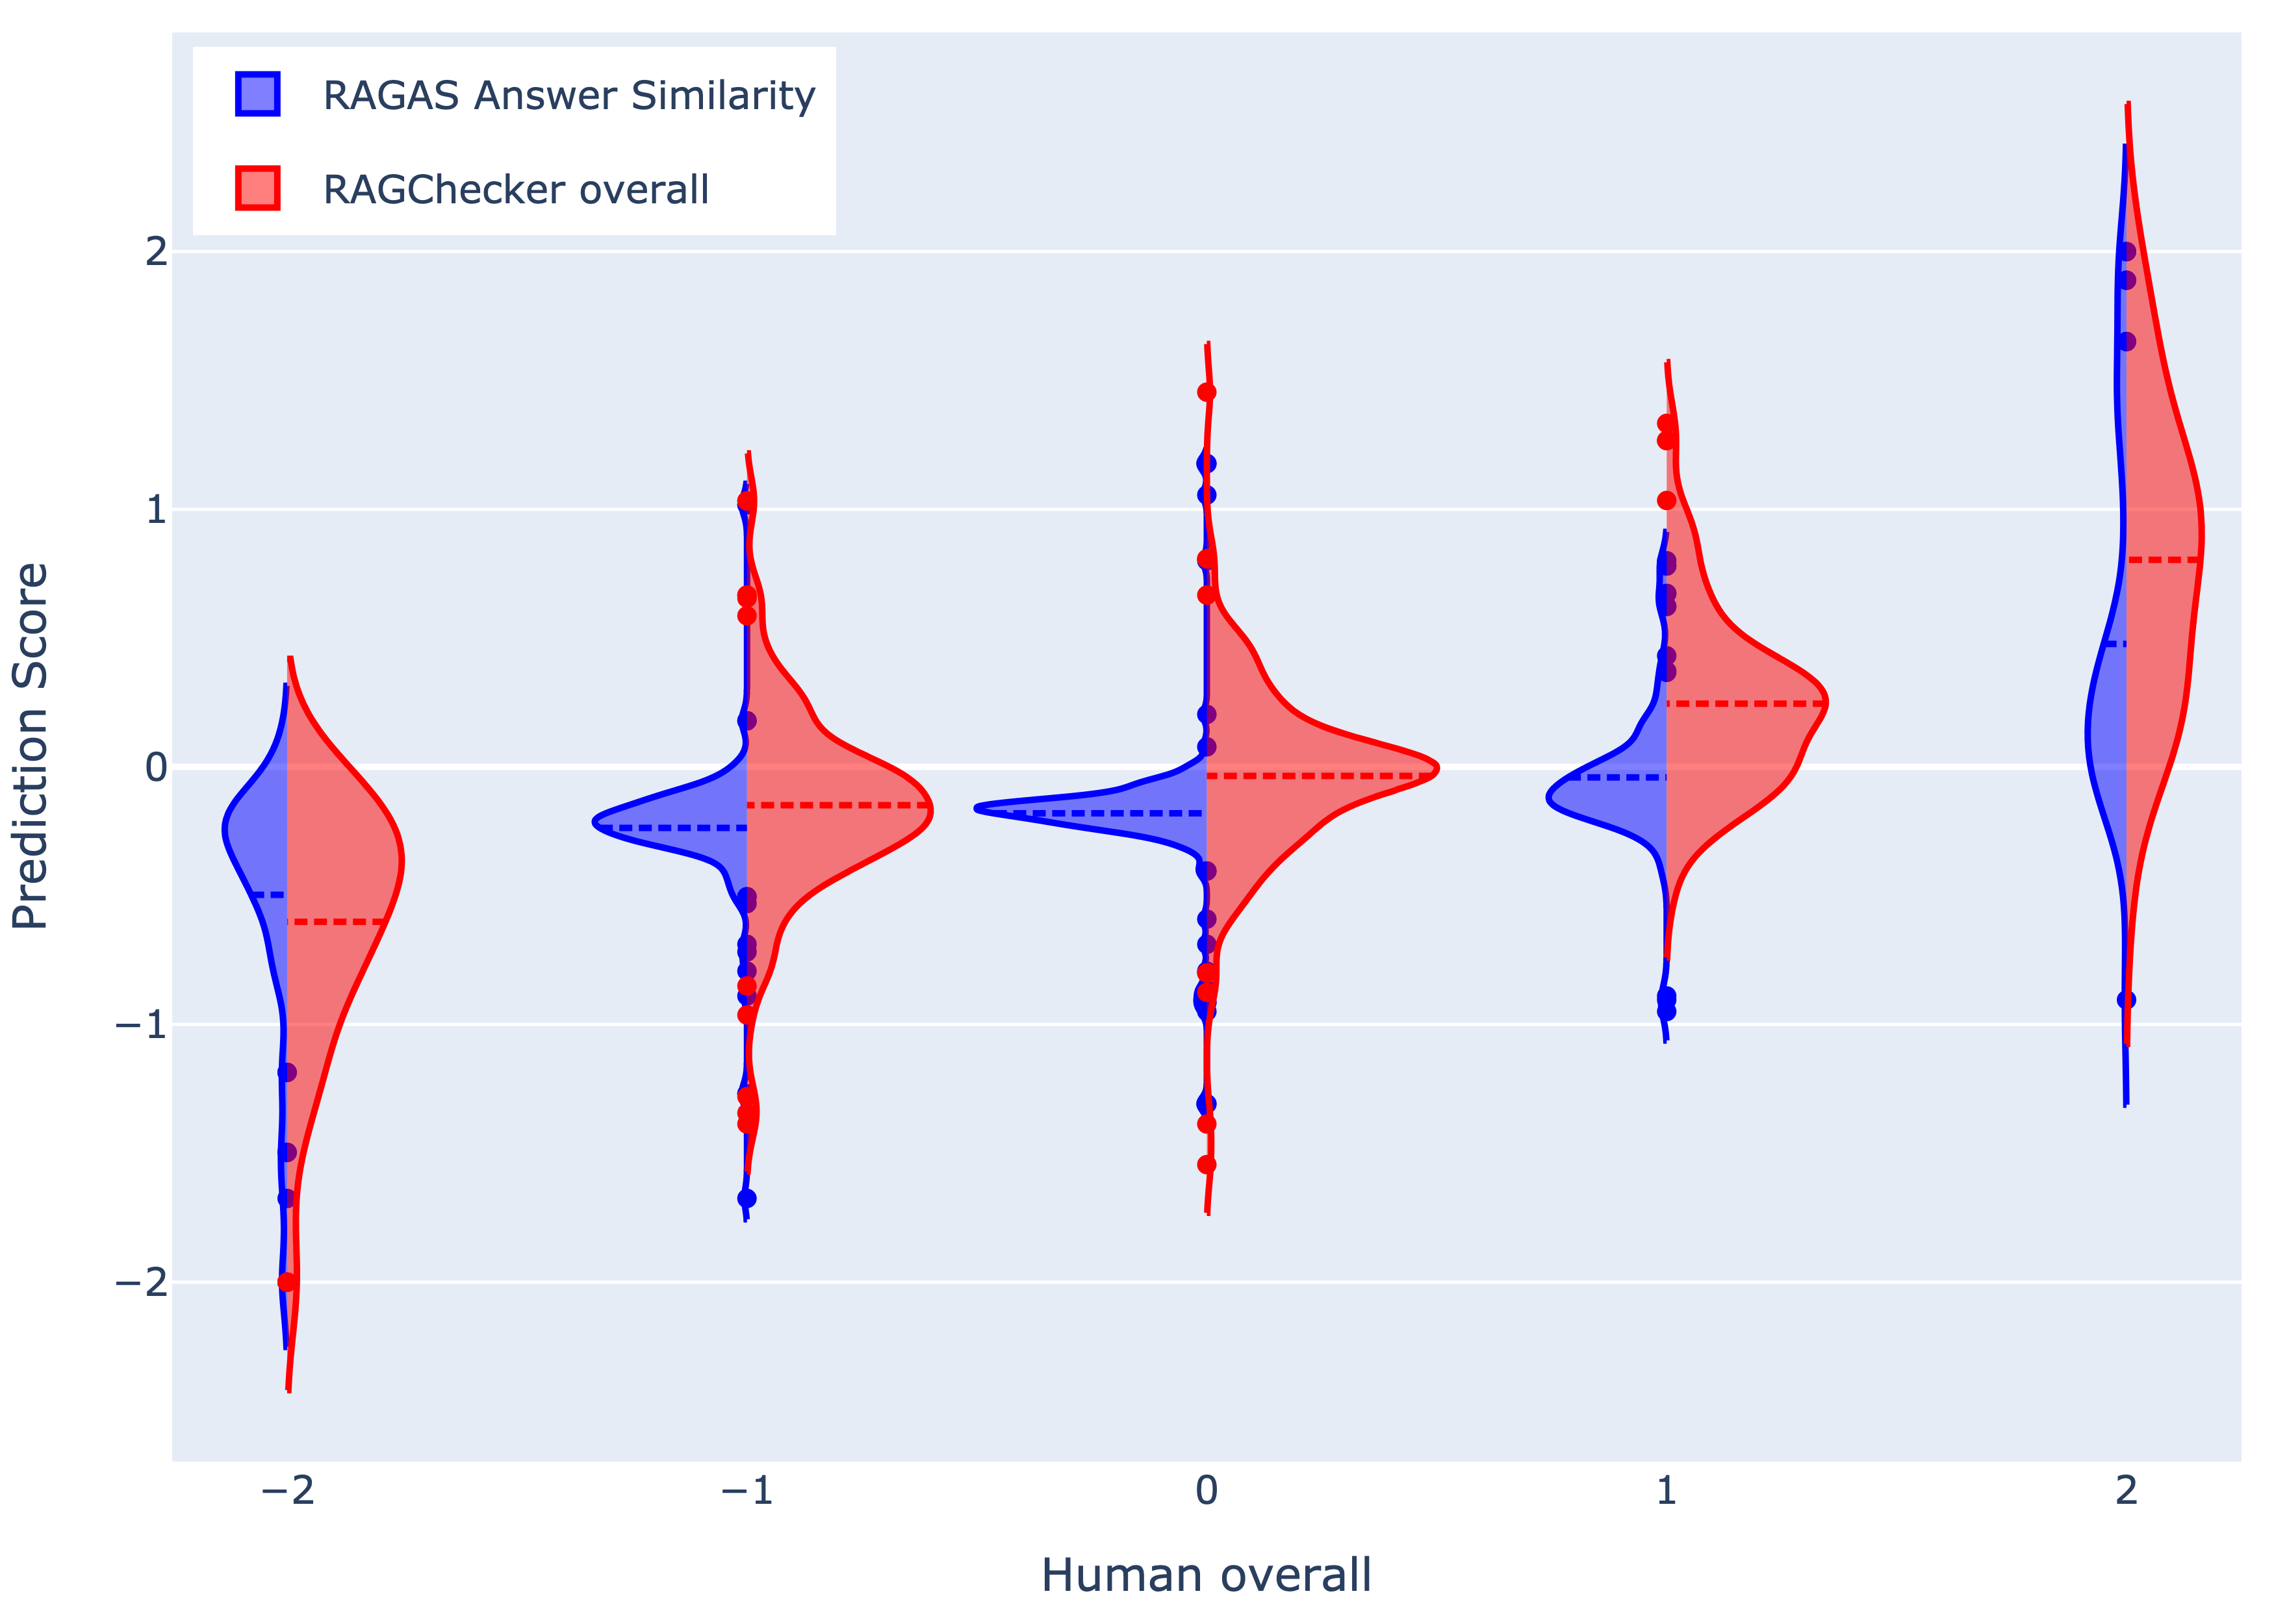
\includegraphics[width=\linewidth]{figures/human_overall.png}
\end{subfigure}
\caption{Comparison of prediction score distribution between \benchname\space and RAGAS Answer Similarity. Each point in the plot represents an instance in the meta evaluation dataset, where the x-axis is the human preference label under corresponding aspect and y-axis is the prediction score of \benchname\space and RAGAS Answer Similarity. The distribution of prediction score is represented by the colored area and the dashed line is the mean line.}
\label{fig:ragchecker_vs_ragas}
\end{figure}